\subsection*{Writing 1, Exercise 6}
The illustration~\ref{fig:ielts_writing_1_8} shows how apple-canning is done. 
Summarize the information by selecting and reporting the main features, and make comparisons where relevant.

\begin{figure}[H]
  \centering
    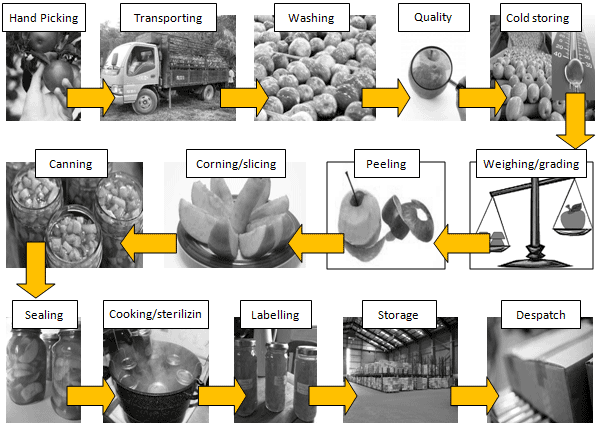
\includegraphics[width=\textwidth]{ielts_writing_1_8}
  \caption{Apple-canning process}
  \label{fig:ielts_writing_1_8}
\end{figure}

\begin{answer}
The diagram shows the process of canning apples step by step. 
Firstly, apples are picked from trees by hand. 
They are then transported to the cannery by large trucks. 
At the cannery the apples are washed and went through a quality check.
The good quality apples are put into cold storage.

When it is ready for canning apples are weighted and graded. 
This step is taken to group fruits by their size. 
After this apples are peeled and sliced. 
Then, apples are put into cans with an addition of apple juice/syrup.

Once the cans have been filled they are sealed and cooked over heat to ensure that the cans are sterilized. 
After sterilizing, cans are labeled and placed into storage.
The canned apples are then dispatched to supermarkets and sold.
\end{answer}
